\chapter{Biomass and Tropical Forests of Southeast Asia}
\chapterauthor{Allison Joseph and Maddie Nelson}
%%%%%%%%%%%%%%%%%%%%%%%%%%%%%%%%%%%%%%%%%%%%
%%% COPY AND PASTE EVERYTHING BELOW THIS %%%
%%%%%%%%%%%%%%%%%%%%%%%%%%%%%%%%%%%%%%%%%%%%


\section{Introduction}

The tropical rain forests of Southeast Asia are a part of the earth's oldest existing tropical ecosystems, spanning across Cambodia, Indonesia, Laos, Malaysia, Myanmar, the Philippines, Singapore, Thailand, and Vietnam.  They are believed to be some of the most biologically diverse ecosystems, their biodiversity and richness unparalleled by that of the Brazilian Amazon and African tropical rain forests. 

 Despite this fact, Southeast Asia is losing its forest coverage faster than any other tropical region in the world. It is predicted that Southeast Asia could lose three quarters of its original forests by 2100 and up to 42\% of its biodiversity \citep{sodhi2004southeast}. Scientists fear that the current rate of deforestation could cause these rain forests to completely vanish in a hundred years. Although not all deforestation is intentional, some resulting from natural factors like wildfires, human impacts and involvement have caused a disproportionate amount of destruction. Most notoriously, the region's forests are endangered and threatened by conversion to agriculture, logging (both legal and illegal), and encroaching oil palm plantations. The human impacts on the rain forests in Southeast Asia have driven many endemic tropical plant and animal species to the brink of endangerment and even extinction. 
 
  Understanding the varied impacts of deforestation are complex, however, this chapter will focus on the formation and destruction of forest biomass in Southeast Asia, a critical component of tropical ecosystems. The presence of forest biomass is essential to the existence of plants, animals and atmospheric processes. Forest biomass greatly influences the global carbon cycle, bio-geochemical processes, and biodiversity.  In addition, forest biomass serves as a habitat for millions of species. However, destruction of forest biomass ultimately alters the interactions between the land surface and the atmosphere, disrupting healthy ecosystem structure and functioning. 

\subsubsection {What is Forest Biomass?}

  \textbf{Biomass} can be defined as the total amount of above ground organic matter in trees, including twigs, leaves, branches and bark. It is referred to as biomass density when expressed as mass per unit area \citep{brown1991biomass}. 

\section {Formation of Biomass}

  Biomass production depends on the environmental factors that influence the course of physiological processes within plant growth. Although many questions remain to be answered regarding the complex chemistry of biomass growth, simply stated, biomass contains energy first derived from the sun. 
  
  \subsubsection{Photosynthesis}
  
  Plant biomass originates by conversion of solar energy and its use in the photosynthetic processes of plants. Through the process of \textbf{photosynthesis}, chlorophyll present in plants absorbs light energy the from the sun. Chemical energy is then created, as the carbon dioxide present in air and water from the ground is transformed into energy-rich organic compounds \textbf{(See Fig. 1.1)}. The majority of light captured by the plants contains wavelengths between the visible and near infrared portions of the electromagnetic spectrum� 400 to 1100 nm \citep{stenberg2010visible}. The light-absorbing pigments that are effective in photosynthesis have absorption bands in this range.
  
   \begin{figure}[ht]
    \centering
        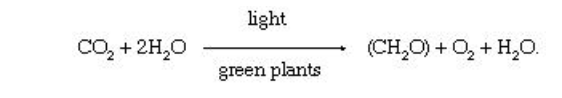
\includegraphics[width = 0.55\textwidth]{graphics/photosynthesisequ.png}
    \end{figure}
    
    Eventually, the same energy that was previously captured from the sun by these plants is released through heat. This process allows for the continuation of plant growth, serving as the the ultimate source of biomass production in ecosystems. Thus, the quantity of biomass in a forest is a result of the difference between production (through photosynthesis) and consumption (by respiration and harvesting processes).
  
  
  
  \begin{figure}[ht]
    \centering
        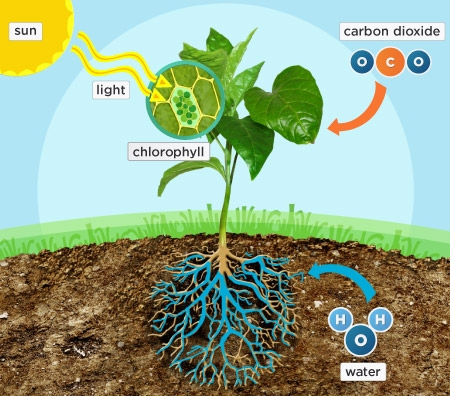
\includegraphics[width = 0.55\textwidth]{graphics/photosynthesis.jpg}
        \caption{The process of photosynthesis.}
    \end{figure}
    

\begin{problem}
  Plants need water, carbon dioxide, and light for photosynthesis. According to the diagram, how does the plant absorb water for photosynthesis? 
\begin{enumerate}[(a)]
    \item Through the leaves
    \item Through the chlorophyll
    \item Through the roots
    \item Through the sun
\end{enumerate}  


\end{problem}

Answer: C

\begin{problem}
According to the diagram, where does the plant get the energy that powers photosynthesis?
\begin{enumerate}[(a)]
\item From chlorophyll
\item From sunlight
\item From carbon dioxide
\item From water
\end{enumerate}  

Answer: B
\end{problem}

\subsubsection {Temperature}
	Aside from the sun, the abundance of biomass in forests is influenced by many factors, such as soil humidity, soil and air temperature, solar radiation, precipitation and soil nutrient availability. One of the most important factors influencing biomass is temperature. Optimum temperatures for plant growth are dynamic since they change with the species and varieties, duration of exposure, age of the plant, and stage of development\citep{marshall1988environmental}. However, the important plant metabolic processes, such as photosynthesis, are influenced by the temperature. Temperature also influences the absorption of water and nutrients, which ultimately affects the plant growth. In addition, soil nutrient availability is another factor influencing plant growth. Both nutrient deficiency and toxicity negatively affect total biomass and fruit production \citep{chatzistathis2013soil}. Thus, by controlling the optimum levels of nutrient availability in soil, the production of biomass can be maximized. In the cases of limited nutrient availability in soils, fertilization is a common practice adopted by the farmers in order to ameliorate the low nutrient status. 

\subsubsection {Geology}
	The high species richness and endemism in Southeast Asia is linked to its complex geological history \citep{sodhi2004southeast}. The tropical forests of Southeast Asia are the oldest, consistent rain forests on Earth, dating back to the Pleistocene Epoch 70 million years ago \cite{hutchison1989geological}. During this formation period, the rest of the world went through cooling and warming periods, but the climate of the Southeast Asian region remained more or less the same. This was due mainly because of its location on the equator and being surrounded by water. Because the climate on the equator does not change much and the surrounding oceans provide plenty of moisture in the form of rain, the region was able to have consistent forests over very long periods of time. 

  As sea levels rose and fell through warming and icing cycles, small pockets of forests survived as reservoirs of wildlife from which various species could re-establish themselves \textbf{(See Fig. 1.2)}. When the glaciers melted and sea levels rose many of these reservoirs were cut off from each other. This forced species to developed their own distinctive evolutionary paths in response to local environments, leading to an amazing diversity of species of every kind.
  
  
   \begin{figure}[ht]
    \centering
        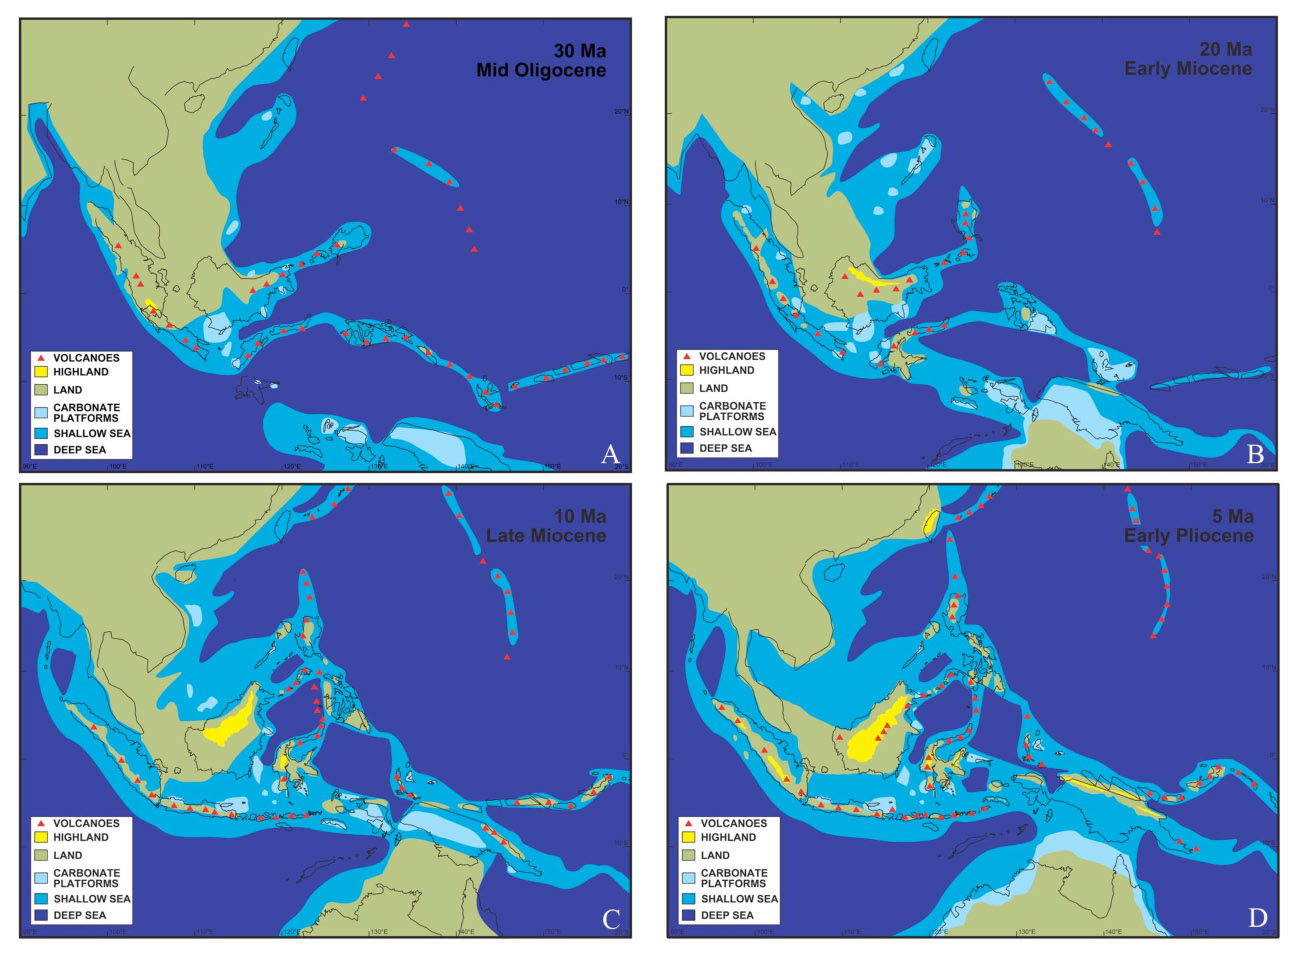
\includegraphics[width = 0.55\textwidth]{graphics/geology.jpg}
        \caption{Postulated distribution of land and sea in Southeast Asia in the Cenozoic. A. 30 mya. B. 20 mya. C. 10 mya. D. 5 mya. Figures from \cite{hall2002cenozoic}.}
    \end{figure} 



\section {Biomass and the Carbon Cycle}

 Studies of the flow of energy and matter have acquired new urgency over the last decade in the response to the need to understand the potential role of natural ecosystems in the mitigation of anthropogenic carbon emissions.

\subsubsection {Carbon and Energy}

   Carbon, in its many forms, is exchanged among the atmosphere, oceans, and land. This is called the carbon cycle \textbf{(see Fig. 1.3)}. A critical part of the carbon cycle takes place in forests. Forests exchange large amounts of CO2 and other gases with the atmosphere and store carbon in in their leaves, wood, and roots. The carbon stored in the plants and soils is called \textbf{sequestered carbon}. The carbon that is returned to the atmosphere when it has been used by trees or other organisms as energy for life is called \textbf{respired carbon}. 
  
    \begin{figure}[ht]
    \centering
        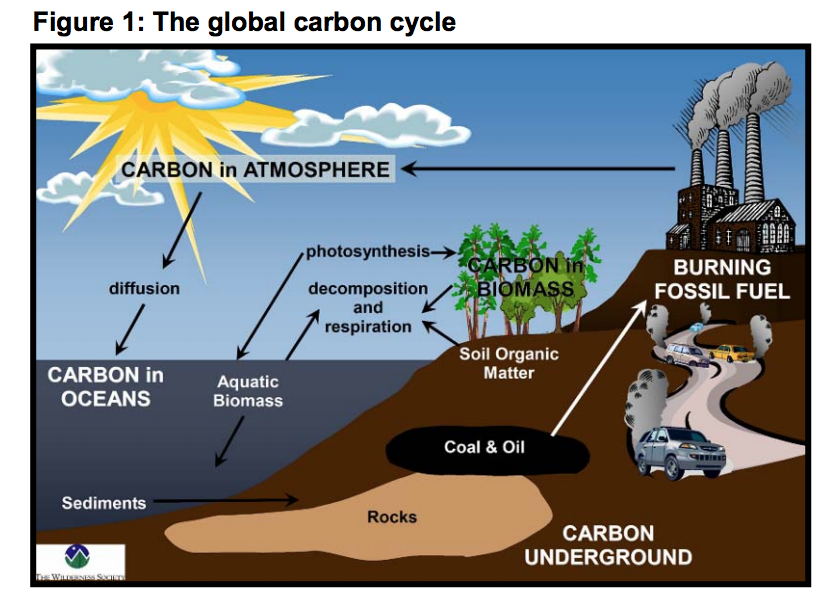
\includegraphics[width = 0.55\textwidth]{graphics/carboncycle.png}
        \caption{The Carbon Cycle. Plants take carbon dioxide (CO2) from the atmosphere and turn it into biomass (wood, leaves, fruits etc.) through photosynthesis. By extracting fossil fuels (oil, gas and coal) from deep in the Earth, we are overloading the atmosphere with carbon, and changing our climate in irreversible ways. In addition, changes in land use, such as deforestation for agriculture, represent a smaller fraction, roughly 15\%, of CO2 emissions each year. Source The Wilderness Society}
    \end{figure}


\subsubsection {Primary Production}

  The importance of forests in the carbon cycle depends on the extent of the forest, the amount of carbon stored per unit area (as plant body or as organic material in the soil), and the rate at which carbon is ``fixed'' by the plants during photosynthesis. The rate of fixation of carbon by photosynthesis is the \textbf{gross primary productivity (GPP)}. Some fraction of this fixed energy is used by primary producers for cellular respiration and maintenance of existing tissues. The remaining fixed energy is referred to as \textbf{net primary production (NPP)}. NPP is the rate at which all the plants in an ecosystem produce net useful chemical energy. It is equal to the difference between the GPP and the rate at which they use some of that energy during respiration\citep{corlett2014ecology}. 

\begin{figure}[ht]
    \centering
        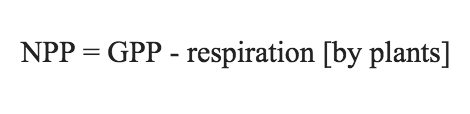
\includegraphics[width = 0.55\textwidth]{npp.png}
    \end{figure}

  The ratio of NPP to GPP - the carbon-use efficiency - is widely assumed to be around .5, but there is evidence to suggest it varies over a wider range \citep{delucia2007forest}. Some, but not all components of the total NPP can be measured directly. Field studies usually measure the two largest components: the above-ground biomass increment (the increase in the dry mass of above-ground plant parts over a measurement interval of one to several years), and the fine litter fall (the dry mass of above-ground plant parts that is produced and shed during the measurement interval for the biomass increment) \citep{ruimy1996turc}. 
  
  
  
  The tropical forests of Southeast Asia account for about one-fifth of the world's forest, and cover around 26\% of the land area in the region \textbf{(See Fig. 1.4)} \citep{brown2003state}.These ecosystems are characterized by vertical layering of vegetation and the formation of distinct habitats for animals within each layer. On the forest floor is a sparse layer of plants and decaying plant matter. Above that is an understory of short, shrubby foliage. A layer of trees rises above this understory and is topped by a closed upper canopy the uppermost overhead layer of branches and leaves.
  
  Although tropical rainforests form less than half of the total forest on earth, their leaf systems comprise approximately 70\% of the world�s total leaf surface area \citep{gower1999direct}. In addition, the temperature and and sunlight profiles of tropical rainforests are stable in comparison to other terrestrial biomes. Their location on the equator provides more solar radiation and therefore more opportunity for primary productivity. Overall, a consistent amount of daily sunlight and lack of temperature seasonality allows for year-round growth.   It is not surprising, then, that tropical rainforests account for between 30\% and 50\% of net primary productivity in terrestrial systems, although they cover only 6\% of the total land area of the earth \citep{houghton2005aboveground}. This means that they store more carbon per unit area than any other type of ecosystem. Thus, tropical forests are critical ecosystems in mitigating the carbon cycle of the planet. 
  
 
 \begin{figure}[ht]
    \centering
        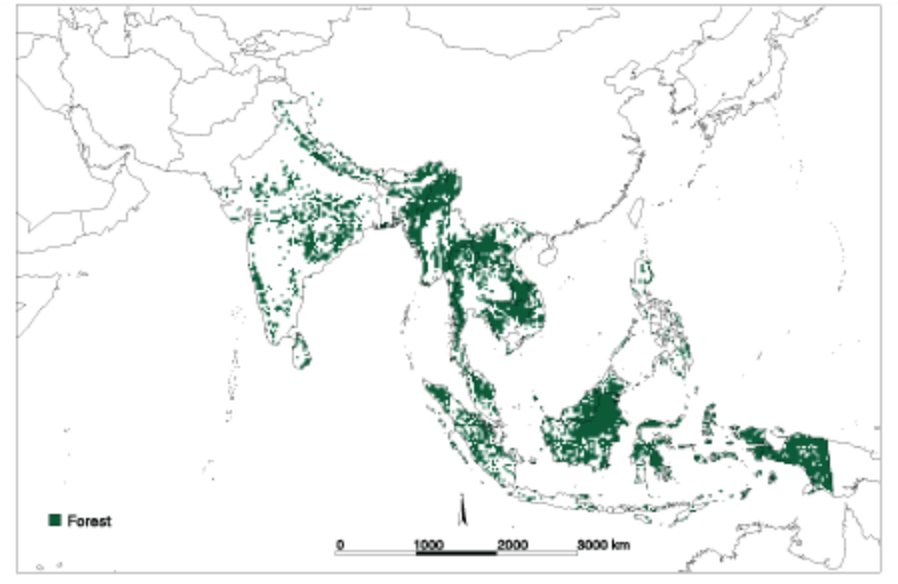
\includegraphics[width = 0.55\textwidth]{graphics/forestcover.png}
        \caption{Forest/non-forest classification of the study area, displayed with 0.25-degree resolution. A database was generated of estimates of geographically referenced carbon densities of forest vegetation in tropical Southeast Asia for 1980. A geographic information system (GIS) was used to incorporate spatial databases of climatic, edaphic, and geomorphological indices and vegetation to estimate potential (i.e., in the absence of human intervention and natural disturbance) carbon densities of forests. The resulting map was then modified to estimate actual 1980 carbon density as a function of population density and climatic zone. \citep{brown1991biomass}.}
    \end{figure}




\section{Deforestation} 

Unfortunately, the tropical forests of Southeast Asia are constantly changing as a result of harvesting and conversion to other land cover. Since the East Asian Miracle in 1990, the FAO (Food and Agriculture Organization) estimates that 38.7 million hectares of primary and other naturally regenerated forest have been lost in the Asia Pacific region � an area greater than the size of Japan \textbf{(See Fig. 1.5)} \citep{faoun163agriculture}. The rapid socio-economic development in Southeast Asia particularly infrastructure, agriculture and industrial development has affected the level of timber production and other forest ecosystem services. In addition, this loss of forests has a profound effect on the global carbon cycle. Tropical deforestation accounts for at least a quarter of all anthropogenic carbon emissions, with both the highest rates of deforestation worldwide and, as a result of high forest biomass, the highest carbon emissions per hectare cleared \citep{corlett2014ecology}.

    \begin{figure}[ht]
    \centering
        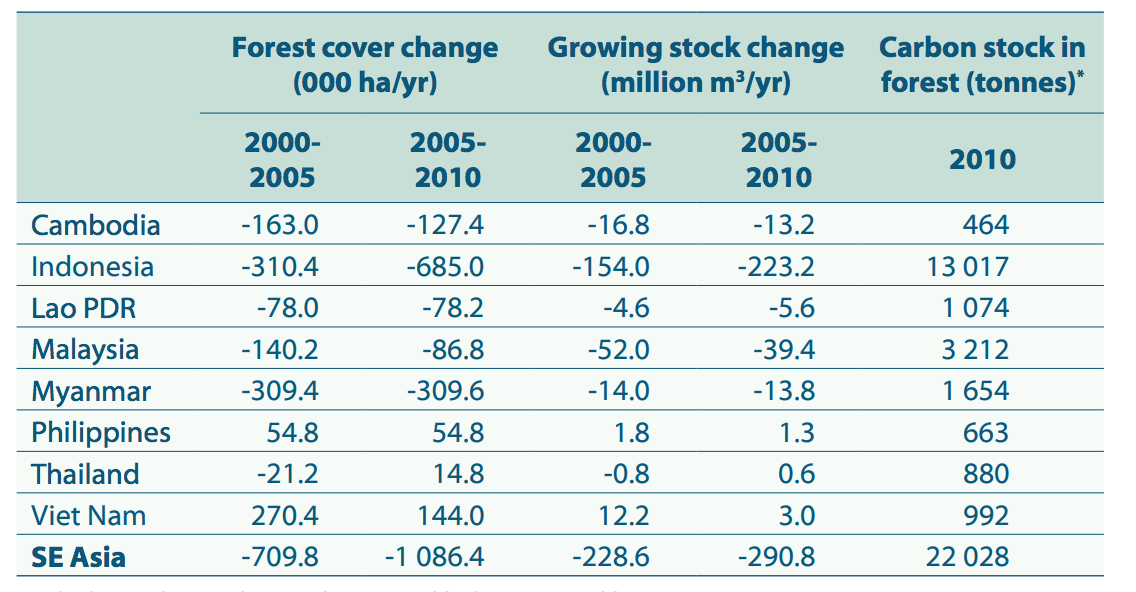
\includegraphics[width = 0.55\textwidth]{graphics/carbonstock.png}
        \caption{Deforestation and degradation rates in Southeast Asian countries, 2000-2010. Includes carbon in living above- and below ground biomass. Source: \citep{faoun163agriculture}.}
    \end{figure}

\subsubsection {Agriculture}
Deforestation occurs in many ways. Most of the clearing is done for agricultural purposes - both grazing cattle and planting crops. Often poor farmers chop down a small area (typically a few acres) and burn the tree trunks, a process known as Slash and Burn agriculture. Intensive, or modern, agriculture occurs on a much larger scale, sometimes deforesting several square miles at a time.

\subsubsection{Palm Oil Plantations}
Found in everything from shampoo to donuts, palm oil is now the most common vegetable oil in the world�and also one of the world's leading deforestation drivers. The large majority of palm oil production occurs in just two countries, Malaysia and Indonesia, where huge swaths of tropical forests have been cleared to make way for oil palm plantations. This transition is responsible for releasing large quantities of carbon into the atmosphere while shrinking habitats for a multitude of endangered species. Between 2000 and 2010 palm cultivation in Malaysia was responsible for 2 to 9 percent of worldwide emissions from tropical land use \citep{carlson2013refined}. 


\subsubsection {Logging} Commercial logging is another common form of deforestation. Logging can occur selectively - where only the economically valuable species are cut  -or by clear-cutting, where all the trees are cut. Logging activities are responsible for at least 50\% decline in the Southeast Asia�s forest carbon density \citep{hawthorne2011impact}. Logging affects the ecological processes in timber concessions by removing biomass, manipulating forest structural characteristics, changing light regimes, and altering microclimatic conditions at both the ground and canopy levels. Logging also introduces people into the forest, increases access via logging roads, and generally increases disturbance. 


\subsection{Sociopolitical Forces}

The motivators for deforestation are very complex. A competitive global economy drives the need for money in economically challenged tropical countries. At the national level, governments encourage modern agriculture or sell logging concessions to raise money for projects, to pay international debt, or to develop industry. The logging companies seek to harvest the forest and make profit from the sales of pulp and valuable hardwoods such as mahogany. Similarly, palm oil plantations or large cattle pastures often replace rainforest to sell their commodities in the world market. 

\subsubsection {Monocultures of the Mind}
South Asian scholar, Vandana Shiva, emphasizes that the regions transition towards industrialism and economic productivity has materialized as traditional local knowledge values of the forest have been systematically undermined \citep{shiva1993monocultures}. This knowledge and power nexus has largely arose in the context of globalization and its associated set of values based on commercial capitalism \citealp{king1993politik}.

This transition is best illustrated in the dominant knowledge and practise of forestry and agriculture. Most local knowledge systems have been based on the life-support capacities of tropical forests, not on their commercial timber value. Traditional food systems based on the forest, either directly, or indirectly have been seen as non-existent in the field of vision of a reductionist forestry and a reductionist agriculture even though they have been and still are the sustenance base for many communities of the world. For example, the rainforests of Southeast Asia supply all the food needs of the Kavan, Kenyah, the Punan Bah, the Penan who gather food from the forest and practise swidden agriculture (1999). The plant supplies are gathered mostly from the surrounding forest, and some 223 basic plant types are regularly consumed. The most important food items are mushrooms (kulat), ferns (paku) and the hearts of various plants (ubot) which include bamboo shoots, wild palms, and wild bananas \citep{hong1987natives}.

Deforestation has been happening for centuries on a smaller scale. However, since the introduction of modern forestry and agriculture, plant biomass has been split into separate non-overlapping domains on the basis of separate commodity markets to which they supply raw materials and resources. In local knowledge systems, the plant world is not artificially separated between a forest supplying commercial wood and agricultural land supplying food commodities. The forest and the field are in ecological continuum, and activities in the forest contribute to the food needs of the local community, while agriculture itself is modelled on the ecology of the tropical forest. In this model, some forest dwellers gather food directly from the forest, while many communities practise agriculture outside the forest, but depend on the fertility of the forest for the fertility of agricultural land. In contrast, the global capitalist industrial complex splits forestry from agriculture and reduces forestry to timber and wood supply \citep{de1989economic}. The creation of fragmented categories thus blinkers out the entire spaces in which local knowledge exists - knowledge which is far closer to the life of the forest and more representative of its integrity and diversity.



 

\section {Biomass and Biodiversity}  

 As these ecosystems have been disrupted, Southeast Asia�s loss of forest biomass has had significant impacts on levels of biodiversity. \textbf{Biodiversity} is defined as the variety of life and its processes, including genes, species, communities, ecosystems and the ecological and evolutionary processes that keep them functioning \citep{noss1994saving}. 
 
 Biodiversity is dependent on the presence of biomass in an ecosystem, studies finding diversity to be positively correlated with the increased presence of biomass \citep{cardinale2007impacts}. Southeast Asian forest biomass provides habitat for a diverse array of organisms, including thousands of vertebrate, invertebrate, lichen and fungi species. These species interact with each other and the environment, providing a diverse array of important ecosystem functions and services . Examples of ecosystem functions that depend on the presence of biomass include soil organic matter supply, contributions to soil development and productivity, and nitrogen fixation \citep{humphrey1999relationships}.
 
 The balance among the many factors sustaining these environments has been increasingly threatened over the last century, as Southeast Asia has lost large percentages of biomass and species diversity.  Over the last 15 years alone, 14.5\% of the region�s forest cover has been destroyed \citep{gullison2007tropica}.  In countries like the Philippines, where deforestation has leveled 93\% of the country�s original forest cover, there is little left to be saved \citep{sodhi2004southeast}. Vietnam has suffered the highest rate of forest destruction in recent decades, losing 43 percent of their forest cover, according to an analysis of satellite imagery. The scope of biomass loss and deforestation was highlighted by the conservation group the World Wildlife Fund (WWF), which noted that from 1973, near the end of the Vietnam War, to 2009, the greater Mekong region lost nearly one-third of its remaining forest cover \citep{sunderland2012evidence}. The impacts of this devastation are substantial in one of the world�s biodiversity hotspots, as there has been large decreases in biomass quantities and available habitats for species. Most remaining forests exist in relatively small and isolated fragments, allowing only the most adaptable species to survive.
 


 \begin{figure}[ht]
    \centering
        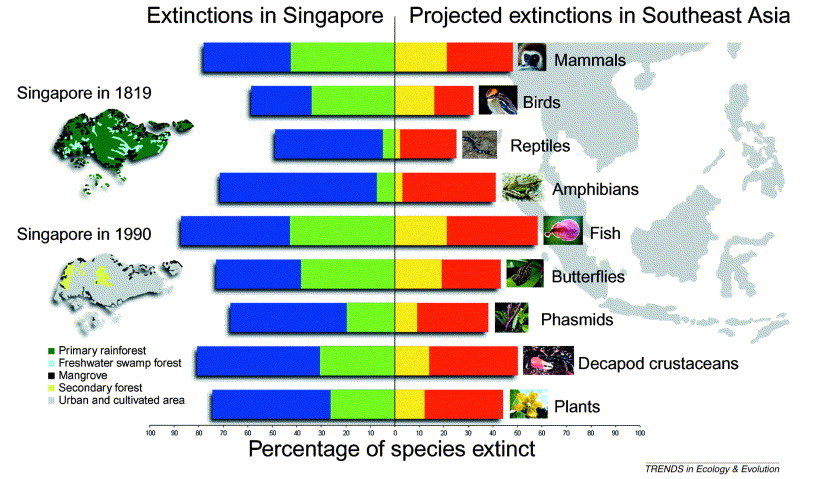
\includegraphics[width = 0.55\textwidth]{graphics/extinction.jpg}
        \caption{This figure illustrates the population extinctions in Singapore and Southeast Asia. Green and blue bars represent recorded and inferred extinctions in Singapore, respectively. Yellow and red bars represent minimum and maximum projected extinctions in Southeast Asia, respectively. \citep{sodhi2004southeast}}
    \end{figure}




\begin{problem}
What is the effect of biomass on ecosystem biodiversity?
\begin{enumerate}[(a)]
\item Biomass has no impact on biodiversity.
\item Increased biomass results in high rates of biodiversity.
\item Increased biomass results in lower rates of biodiversity 
\end{enumerate}
\end{problem}

\begin{problem}
The fragmentation of forests:
\begin{enumerate} [(a)]
\item Increases the number of species, reducing competition for food resources
\item Creates isolated habitats, upon which species biodiversity increases
\item Decreases biodiversity, allowing only the most adaptable species to survive
\item Is a preferred method of forest conservation
\end{enumerate}
\end{problem}

\begin{problem}
True or False: Mono-culture forests produce higher rates of above ground biomass than mixed species forests.

False. Mixed species forests produce higher rates of above ground biomass and biodiversity.
\end{problem}


\subsubsection{Case Study: The Javan Rhinos}

  Large mammals, such as the Javan rhino, are especially vulnerable to forest degradation because they require large areas of forest to survive. The Javan Rhino is a herbivore, whose source of food depends on lowland rainforest biomass. The Javan rhino is primarily a browser,  its diet consisting of shoots, twigs, young foliage and fallen fruit. 

 The Javan Rhino was declared extinct in Vietnam in 2010, due to the compounding effects of poaching and deforestation \citep{brook2014lessons}. In addition to inadequate response to heavy poaching of rhinos, forest habitats well-suited to rhinos were disproportionately impacted by deforestation and fragmentation for agricultural plots.  Conservation efforts, which commenced in earnest during the late 1980s, proved too late for the Javan Rhino.  It is now the hope that lessons learned from the Vietnamese population of rhinos may be used to protect the remaining population in Indonesia.
  
   \begin{figure}[ht]
    \centering
        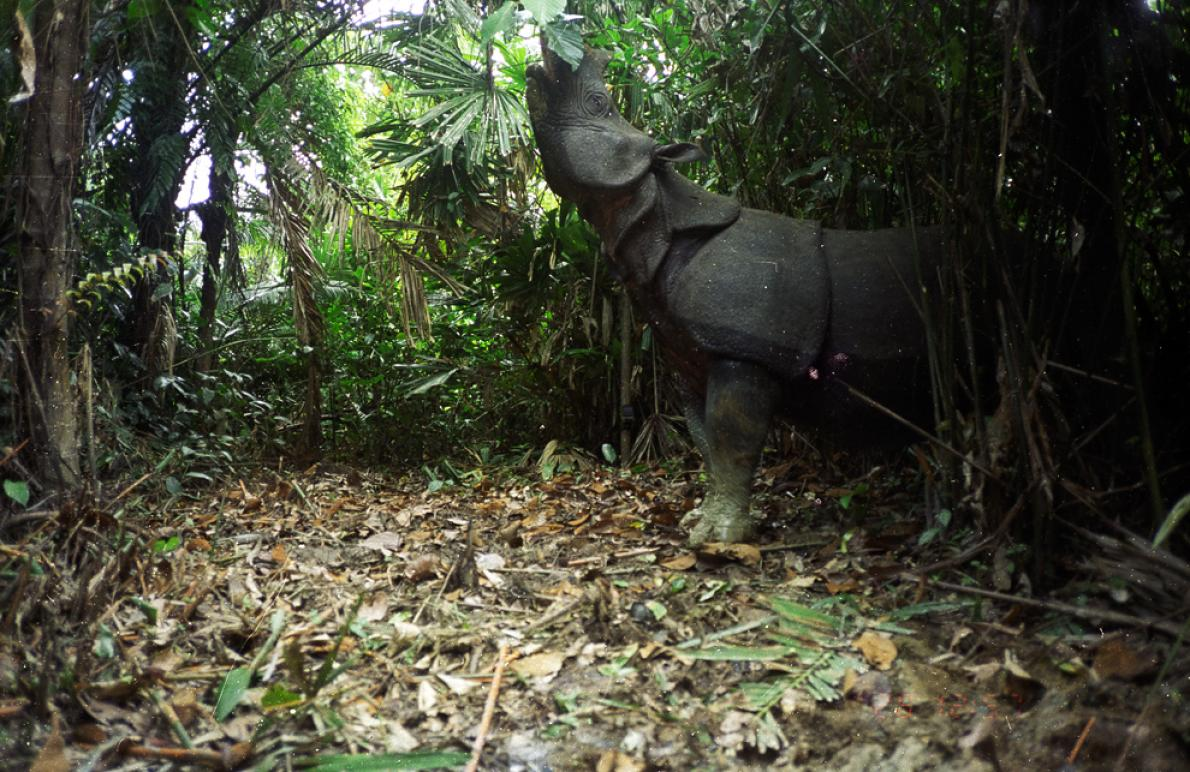
\includegraphics[width = 0.55\textwidth]{graphics/javan.jpg}
        \caption{This figure illustrates the population extinctions in Singapore and Southeast Asia. Green and blue bars represent recorded and inferred extinctions in Singapore, respectively. Yellow and red bars represent minimum and maximum projected extinctions in Southeast Asia, respectively. \citep{sodhi2004southeast}}
    \end{figure}

  
  The remaining Javan rhinos live within the Udung Kulon National Park, located on a small Indonesian Island. Although protected, the park and its surrounding forests are under pressure from human activities. In addition, the rhinos find themselves threatened by the invasive Arenga palm, which is having a devastating impact on the plants that the rhinos rely on for food. The palm has spread to cover more than half of the area inhabited by rhinos, shading out the under-story and reducing the amount of plants available to the rhinos. This decreased availability of food reduces the carrying capacity of the park and slows the breeding rate of the rhinos.

  Recently, there have been talks of re-locating a small number of the remaining Javan Rhino population and forming a second, independent population.  Conservationists are concerned about the risk of natural disasters on the Indonesian island. Increased tectonic and volcanic activity threaten the rhinos, as well as the compounding threat of tsunamis due to these natural disasters \citep{setiawan2018preventing}.  However, without the appropriate amount of forest space and biomass, the 62 remaining rhinos will not survive in a new location. 

\begin{problem}	
	Discuss:
Is saving the Javan Rhino worth the time, money and effort of conservationists? Why or why not? 
\end{problem}


\subsection{Conservation and Forest Management}

The complexity of addressing the threats facing Southeast Asian tropical forests have made the region a top conservation priority. However, environmental apathy, corruption, poor natural resource governance, poverty, lack of data, and lack of conservation funding remain formidable challenges for conservationists in Southeast Asia \citep{sodhi2004southeast}.

Scientists of the WWF and other experts believe that it is essential to begin preserving the greater Mekong region�s forest. The Vietnamese government has been heralded for its reforestation efforts, yet, these programs largely consist of monoculture tree plantations that harbor limited biodiversity and decreased biomass. Results of long-term experiments in Southeast Asia have examined the effect of tree species biodiversity on aboveground biomass quantities. Forest mixtures and corresponding monocultures were compared on the same site to control for outside environmental variables such as climate or weather. The study found that the productivity of mixed-species forests was 15\% greater than the average of their corresponding monocultures, and not statistically lower than the productivity of the best corresponding monoculture \citep{sunderland2012evidence}. Thus, the greater biodiversity of mixed species forests produced statistically significant higher rates of above ground biomass.

The presence and continued supply of biomass represents a key concern in managed forest systems  Overall, conservation responses will need to be strategic, addressing the need for long-term development and employing temporary measures to secure species and ecosystems under imminent threat. Future conservation policies will act as living documents in repsonse to the regions they represent. Multiple actions will be needed, ranging from initiatives at international, regional and national policy level to many thousands of projects, negotiations and decisions at the level of sites and landscapes. 

However, the decisions by policy-makers regarding the management and use of forest and trees will require more accurate and precise information on the state and patterns and rates of change of the resource. To attain these needs, reliable estimates on the state and change of forest biomass for all countries over the long term must be made \citep{brown1991biomass}. 



\section{Conclusion}

The tropical forest biomass of Southeast Asia plays an intricate and vital role in the functioning of healthy ecosystems and atmospheric balances. However, tropical deforestation has greatly lowered quantities of forest biomass, resulting in decreased biodiversity, a disruption of ecosystem service and the endangerment of endemic species. In addition, through its essential participation in the global terrestrial carbon cycle, forest biomass has been recognized as an essential climate variable.

Forest biomass also affects global and regional climate and environmental health.  From 2002 to 2012, the degradation of forest was responsible for a 10\% increase in greenhouse gas emissions \citep{gullison2007tropical}. It is estimated that forest protection and reforestation efforts, if successful, could be powerful enough to offset greenhouse gas emissions for up to 40 years as other energy sources are developed and integrated \citep{lasco2002forest}. With booming economies, the countries of the Southeast Asia region must now balance legitimate needs for development while safeguarding ecosystem services that are under growing threat. 

Thus, in the coming decades, the preservation and management of forest biomass should remain a top priority for conservationists, government officials, and local individuals. Many scientists are currently researching the best methods of sustainable forest management, with the hope of developing practical recommendations for a modern Southeast Asia. 
%%%%%%%%%%%%%%%%%%%%%%%%%%%%%%%%%%%%%%%%%%%%
%%% COPY AND PASTE EVERYTHING ABOVE THIS %%%
%%%%%%%%%%%%%%%%%%%%%%%%%%%%%%%%%%%%%%%%%%%%